\chapter{Vorverarbeitung}
Wie in Kapitel X beschrieben, ist es möglich aus den rohen Sensordaten die Rotation und die Position zu jedem Messzeitpunkt zu berechnen. Dieses Kapitel beschreibt diese Umrechnung und etwaige Herausforderungen. Abbildung X zeigt den Ablauf der Berechnung.

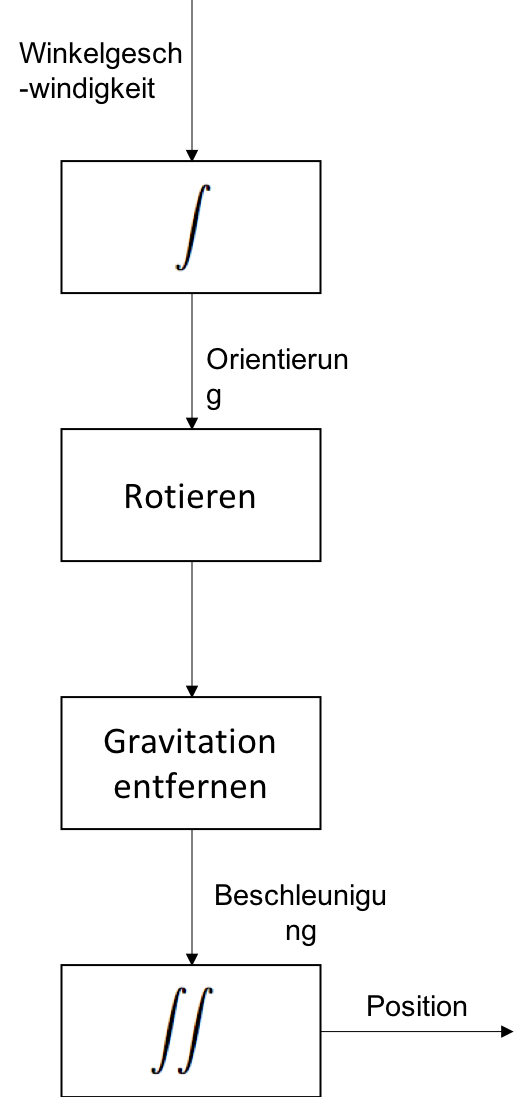
\includegraphics[scale=0.5]{Bilder/WorkflowVorverarbeitung.png}

Wie die Grafik zeigt, ist die Berechnung der Position direkt abhängig von der Berechnung der Orientierung. Gleiches gilt allerdings auch für die Fehleranfälligkeit. Fehler in der Berechnung der Orientierung werden durch die Umrechnung dieser in die Position verstärkt. Daraus folgt, dass sich schlechte Qualität der rohen Sensordaten noch deutlich stärker in Fehlern bei der Position niederschlagen als schon bei der Orientierung. 
\section{Rotationsberechnung}
\subsection{Complentary Filter}

\section{Positionsberechnung}
\subsection{Trapez-Filter}
projektspezifische Anpassungen usw.